\chapter{Estudo das soluções}

\section{Parâmetros avaliados}
Durante o desenvolvimento do projeto, serão analisadas diferentes topologias e soluções para maximizar o desempenho da máquina, considerando parâmetros como frequência natural, rigidez, consumo de materiais e velocidade máxima.

\subsection{Ergonomia}
A máquina foi projetada para facilitar o acesso aos seus componentes e o ajuste manual, quando necessário, considerando a segurança e o conforto do operador.


\subsection{Frequência Natural das Soluções}
O primeiro passo para verificar se a frequência natural de uma máquina está assumindo um valor coerente com a aplicação é comparando-a com a frequência de operação dela. Dessa forma, utilizando uma frequência de operação de 30 MHz --- proveniente dos motores e definida nas especificações de projeto, é preciso garantir que a frequência natural de vibração da solução seja maior que essa. 


Dada a complexidade da estrutura detalhada e da definição de uma equação do movimento que poderia ser proveniente da situação real das guias e das mesas, será utilizado um modelo de simplificação, com algumas hipóteses assumidas. O livro \cite{blevins2001formulas} foi utilizado como base para definição desse modelo estrutural para este cálculo. Assim, a versão simplificada do elemento crítico vibrante --- guia e mesa --- foi considerada como uma barra esbelta com uma massa apoiada no centro. Duas alterativas foram consideradas, representadas na Fig. \ref{fig:blevins-models}.

\begin{figure}[h]
    \centering
    \begin{subfigure}{0.45\textwidth}
         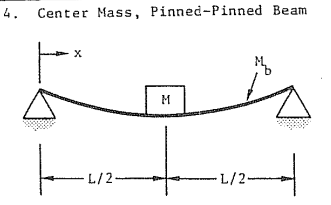
\includegraphics[width=\textwidth]{images/frequencia/center-mass-pinned-pinned.png}
         \caption{Viga bi-apoaiada}
    \end{subfigure}
    \begin{subfigure}{0.45\textwidth}
         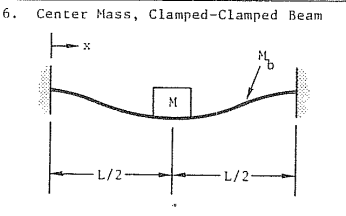
\includegraphics[width=\textwidth]{images/frequencia/center-mass-clamped-clamped.png}
         \caption{Viga bi-engastada}
    \end{subfigure}
    \caption{Modelos de viga esbelta com massa central. Fonte: \cite{blevins2001formulas}}
    \label{fig:blevins-models}
\end{figure}

Para o modelo representado em \ref{fig:blevins-models}(a), a frequência natural pode ser sintetizada pela Eq. \ref{eq:pinned-pinned}, enquanto o modelo em \ref{fig:blevins-models}(b) pela Eq. \ref{eq:clamped-clamped}.

\begin{equation}
\frac{2}{\pi}\left[\frac{3EI}{L^3 (M+0.49M_b)}\right]^{1/2}
\label{eq:pinned-pinned}
\end{equation}

\begin{equation}
\frac{4}{\pi}\left[\frac{3EI}{L^3 (M+0.37M_b)}\right]^{1/2}
\label{eq:clamped-clamped}
\end{equation}

Considerando o pior caso, em que a frequência natural de vibração é menor e, pontanto, mais próxima da frequência mínima limitada pelas especificações do projeto, foi selecionado o modelo da Eq. \ref{eq:pinned-pinned}: a viga bi-apoiada. 

Uma vez selecionado o modelo, é possível estudar a expressão para que sejam especificados os parâmetros utilizados. Destrinchando-os, é preciso conhecer propriedades mecânicas, esturturais e geométricas dos elementos da composição --- guias e a massa móvel:
\begin{itemize}
    \item  E --- módulo de elasticidade do perfil 
    \item I --- segundo momento de inércia do perfil quando uma carga é aplicada e ha deflexão
    \item L --- comprimento do perfil 
    \item M --- massa móvel posicionada no centro do perfil
    \item $M_b$ --- massa dos perfis/guias
\end{itemize}

Adicionalmente, é possível detalhar o momento de inércia  e a massa móvel, definindo-os respectivamente a partir das Eqs. \ref{eq:inertia} e \ref{eq:movel}. O momento de inércia é como o momento de inércia a flexão para duas barras cilíndricas, no caso do eixo das guias. Como a seção é formada for duas barras, deve-se multiplicar o valor de $I$ por dois. Vale ressaltar que esse cálculo pode ser aplicado para as soluções convencionais onde a seção mais propensa a vibração por flexão é a das guias lineares. Posteriormente, na análise de cada uma das soluções, são propostos cálculos de momentos de inércia e massas móveis específicas para cade um dos modelos.  

\begin{equation}
 I = \frac{\pi R^4}{4} 
\label{eq:inertia}
\end{equation}


\begin{dmath}
    M_{\text{móvel}} = (\text{Massa da mesa deslizante})\times 2 + \text{Massa dos perfis da mesa superior} + \text{Massa do porta ferramenta}
\label{eq:movel}
\end{dmath}


A partir dessas expressões, é necessário fornecer o valor de mais parâmetros, sendo eles:
\begin{itemize}
    \item R --- raio dos perfis
    \item $\rho$ --- massa específica do material que compõe o perfil e a mesa (nessa aplicação, esse material é aço)
\end{itemize}


Dessa maneira, é possível determinar, baseado no posicionamento e na escolha das mesa deslizantes assim como sua fixação e adição de massas móveis, qual será a frequência crítica de vibração natural. 

Em adição, é também possível determinar outro tipo de frequência natural de vibração, sendo ela a vibração torsional, que pode ocorrer entre as guias e a mesa. Mas, como essa seria menos menos crítica em relação á frequência de operação, não será limitante para este projeto. 

% de aço = 200 ∗ 109P a
% • L : Comprimento do perfil = 430 ∗ 10−3m
% • Lmesa4 : Comprimento do perfil = 280 ∗ 10−3m
% • R : Raio dos perfis = 10 ∗ 10−3m
% • ρ : massa espec´ıfica a¸co = 7870kg/m3
% • Mb : Massa dos perfis = 2.13kg
% • M : Massa m´ovel = 10.5kg
% • d : distˆancia at´e o eixo = 36 ∗ 10−3m




%% maior rigidez e a da torre -> precisamos determinar a rigidez dele 




%% Frequencia torsional 




% A frequência máxima que vai ser atingida por nossa máquina é 30Hz.(Motores)
% Considerando a rigidez das estruturas das soluções apresentadas, pode-se constatar que os suportes com perfil quadrado em aço de 100mm e 80 mm apresentam um momento de inércia superior ao do perfil da barra delgada da mesa deslizante número 3 que possui 430 mm de comprimento e dois perfis cilíndricos de 20 mm de diâmetro, com um momento de inércia inferior.
% Dessa forma, calculou-se a frequência natural para a mesa deslizante 3 considerando os suportes apresentados nas soluções, biapoiados, e uma massa concentrada no meio dos perfis cilíndricos que corresponde a mesa deslizante de
% número 4, 280 mm, o porta-ferramenta, motor de passo e demais chapas de aço.



\subsection{Rigidez (Loop Estrutural)}
A rigidez estrutural foi analisada para minimizar deformações durante a operação, garantindo precisão e acurácia nas usinagens. O material mole impacta a rigidez.

%%%%%%%%%%%%%%%%%%%%%%%%%%%%%%%%%%%%%%%%%%%%%%%%%%%%%%%%%%%%%%%%


\section{Solução 1}
\begin{figure}[h!]
    \centering
    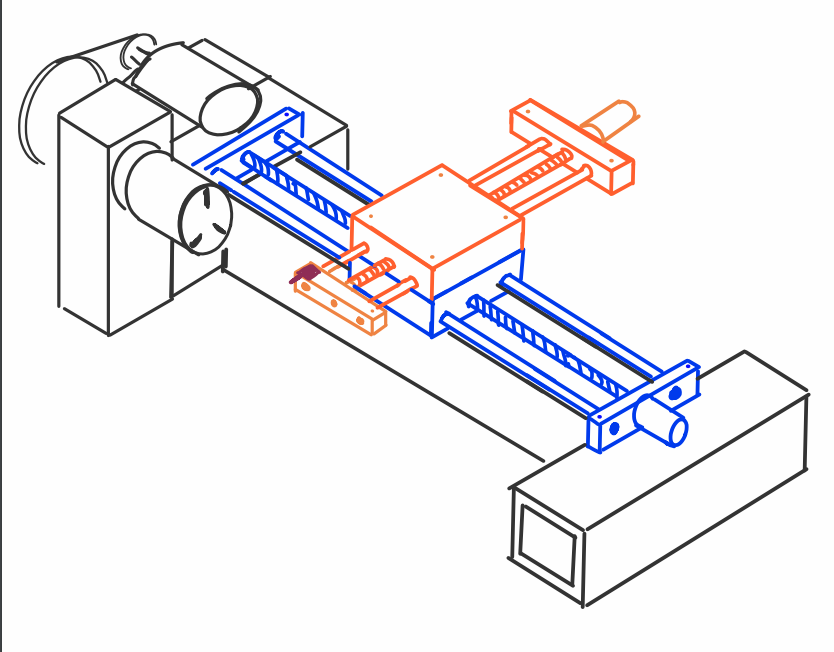
\includegraphics[width=0.7\linewidth]{images/sol1.png}
    \caption{Esboço manual da primeira solução. Fonte: Autor.}
    \label{fig:enter-label}
\end{figure}

\subsection{Peso}

Considerando 3 perfis de 100mmx100mm e tendo como base a estimativa de dimensão: \\
\begin{itemize}
    \item 860mm de comprimento: 8,3kg
    \item 400mm de largura: 3,9kg
    \item 270mm de altura: 2,6kg
\end{itemize}

Com uma chapa de aço 3,2mm entre as mesas considerera-se 290mm de comprimento e 150mm de largura, dimensões suficientes para fixação da guia.  \\
Peso: 0,824 kg \\

Peso extra relacionado a solução 2: 15,7kg \\

\textbf{Peso total:} 40,9kg


\section{Solução 2}

\begin{figure}[h!]
    \centering
    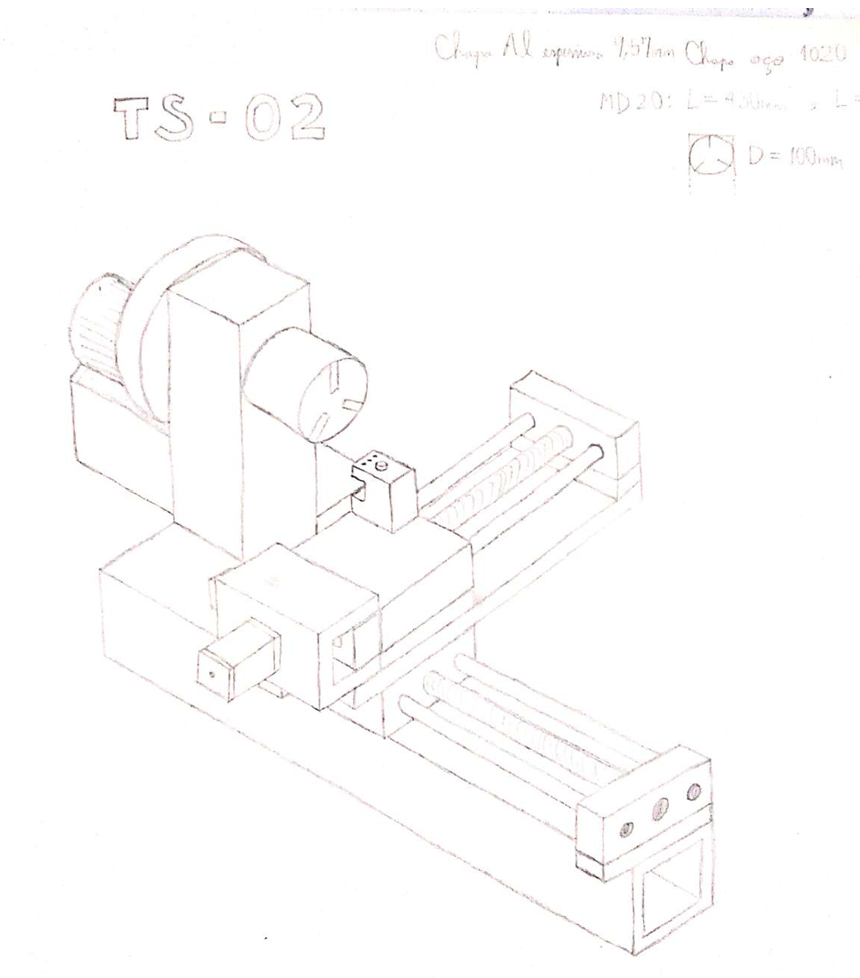
\includegraphics[width=0.7\linewidth]{images/sol2.png}
    \caption{Esboço manual da segunda solução. Fonte: Autor.}
    \label{fig:enter-label}
\end{figure}

\subsection{Peso} 


\section{Solução 3}
\begin{figure}[h!]
    \centering
    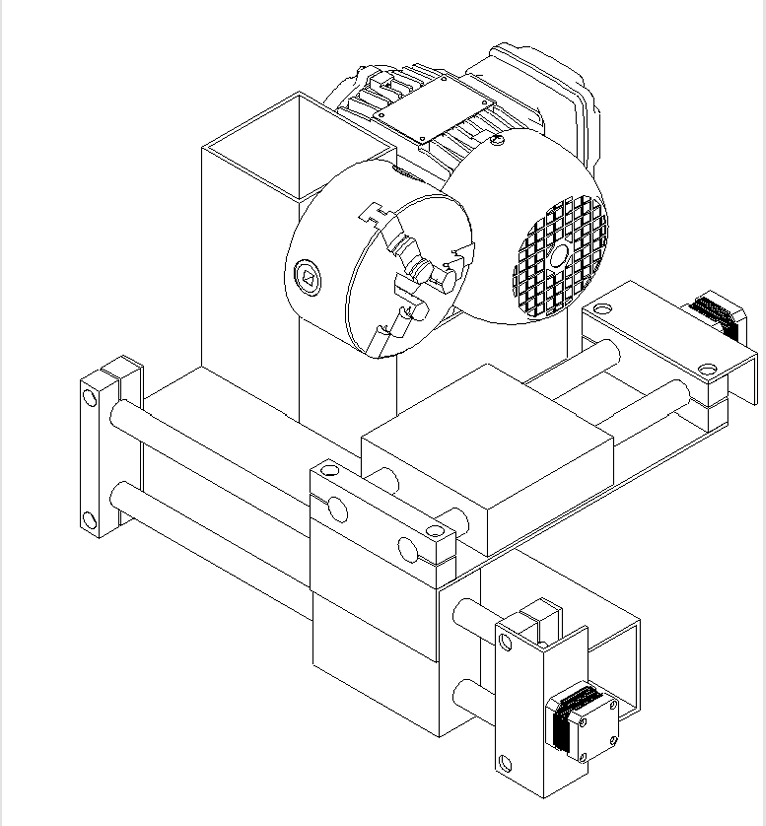
\includegraphics[width=0.7\linewidth]{images/sol3.png}
    \caption{Esboço da terceira solução. Fonte: Autor.}
    \label{fig:enter-label}
\end{figure}

\subsection{Peso}

\begin{itemize}
    \item 2x chapas fixação eixo Z: 0.126 kg
    \item 2x placa motor de passo: 0.586 kg
    \item Eixo árvore: 2.54 kg
    \item Eixo Z : 3.473 kg
    \item Placa mesa de cima : 1.181 kg
    \item Chapa do motor: 0.372 kg 
    \item Base do motor : 1.702 kg
    \item Porta ferramentas: 0.37 kg
\end{itemize}

\textbf{Peso total: }10.35 kg



\section{Matriz de Decisão}

\begin{table}[h]
    \centering
    \begin{tabular}{|c|c|c|c|c|c|c|c|} \hline 
        \multicolumn{2}{|c|}{}& \multicolumn{2}{|c|}{\textbf{Solução 1}} & \multicolumn{2}{|c|}{\textbf{Solução 2}} & \multicolumn{2}{|c|}{\textbf{Solução 3}} \\ \hline  \textbf{Critério}&  \textbf{Peso}& \textbf{Nota} & \textbf{PxN} & \textbf{Nota} & \textbf{PxN} & \textbf{Nota} & \textbf{PxN} \\ \hline  
        Peso & 3 & 3& 9& 5& 15& 3& 9
\\ \hline  
        Rigidez & 7 & 5& 35& 5& 35& 3& 21
\\ \hline  
        Frequência natural & 5 & 3& 15& 5& 25& 1& 5
\\ \hline  
        Velocidade e acelerações & 6 & 3& 18& 5& 30& 3& 18
\\ \hline  
        Erro de Abbe & 3 & 3& 9& 5& 15& 1& 3
\\ \hline  
        Facilidade de montagem & 2 & 3& 6& 5& 10& 1& 2
\\ \hline  
        Facilidade de manufatura & 1 & 3& 3& 5& 5& 3& 3
\\ \hline  
        Segurança do operador & 4 & 1& 4& 5& 20& 5& 20\\ \hline  
 \multicolumn{2}{|c|}{Média Ponderada}& \multicolumn{2}{|c|}{3,35}& \multicolumn{2}{|c|}{4,74}& \multicolumn{2}{|c|}{2,35}\\ \hline 
    \end{tabular}
    \caption{Matriz de decisão entre as soluções propostas.}
    \label{tab:comparativa}
\end{table}

\subsection{justificativa das notas atribídas}

Para todos os critérios, as notas variam de 1 a 5 e procura-se atribuir apenas notas ímpares para as soluções de maneira que haja distanciamento significativo entre as notas medias ponderadas, possibilitando a escolha da solução. 

\begin{itemize}
    \item Peso
    
    Tanto a solução 1 quanto a 3 possuem uma chapa que une a mesa superior à mesa inferior. Por isso, receberam notas menores do que a solução 2. Além disso, o peso adicionado por essa chapa é igual em ambos os casos e não é tão significativo quando comparado ao peso total da máquina para justificar a atribuição de uma nota "1" para as soluções. 
    
    \item Rigidez
    
    A solução 1 e 2 receberam nota máxima nesse quesito, pois é possível identificar que o material a ser uninado seria o ponto mais fraco do laço estrutural. Já para a solução 3 foi atribuída uma nota menor, pois como a ferramenta estaria fixada na ponta da mesa em balanço, a mesa poderia sofrer deformações que afetassem a rigidez da solução.
    
    \item Frequência natural
    
    Dados os modelos de uma viga bi-apoiada para as soluções 1 e 2, e de uma viga com uma das extremidades engastada e a outra em balanço para a solução 3, foram calculadas as frequências naturais de oscilações da estrutura composta pelas guias e mesa deslizantes superiores ads soluções. Assim, as notas foram atribuidas de maneira diretamente proporcional à frequência obtida.

    
    \begin{table}
        \centering
        \begin{tabular}{|c|c|c|c|} \hline 
             Solução&  Frequência [Hz]&  Modo& Nota\\ \hline 
             1&  98&  Flexão& 3\\ \hline 
 2& 102& Flexão&5\\ \hline 
             3&  53&  Flexão& 1\\ \hline
        \end{tabular}
        \caption{Freqências e notas da soluções}
        \label{tab:freq_not}
    \end{table}
    
    \item Velocidade e acelerações
    Como as soluções 1 e 3 possuem maior massa móvel que a 1, foram obtidas para elas acelerações e velocidades máximas menores que para solução 2. assim, elas receberam notas menores
    
    \item Erro de Abbe
    
    O Erro de Abbe foi considerado ao analisar a altura da ferramenta em relação ao seu ponto de fixação na quia ou mesa. Essa metodologia foi escolhida pois quanto maior é o porta ferramentas, maior é a deformação gerada nele por conta das forças de usinagem e maior o erro de Abbe.
    
    \item Facilidade de montagem
    
    Esse critério foi analisado contando o número de peças necessárias para formar a solução. Além disso, a solução 3 recebeu uma nota menor que a 1, apesar de ter o mesmo numero de peças, por ter uma das extremidades em balanço, o que causaria uma dificuldade para alinhamento das estruturas.
    
    \item Facilidade de manufatura
    
    Esse critério foi analisado contando o número de peças necessárias para formar a solução. A solução com menor número de peças recebeu a maior nota.
    
    \item Segurança do operador
    
    As soluções 1 e 2 receberam as mesmas notas, mas a solução 3 recebeu uma nota menor por conta da possibilidade de acidentes que podem ser causados pelas vibrações e deformações excessivas em sua extremidade livre.
    
\end{itemize}
